\subsection{Role within the VO architecture}

The IVOA Provenance Data Model is structuring and adding metadata to trace the
original process followed during the data production for providing astronomical
data. Even if it borrows the main general concepts from data
management science, it binds to the specific context of astronomical metadata
description and re-uses or interacts with existing IVOA models. It takes
benefits from existing IVOA notations and standards like UCD, VOUnits, VO
protocols and service design; and it is planned for a full integration into the
VO landscape.

\begin{figure}
\centering
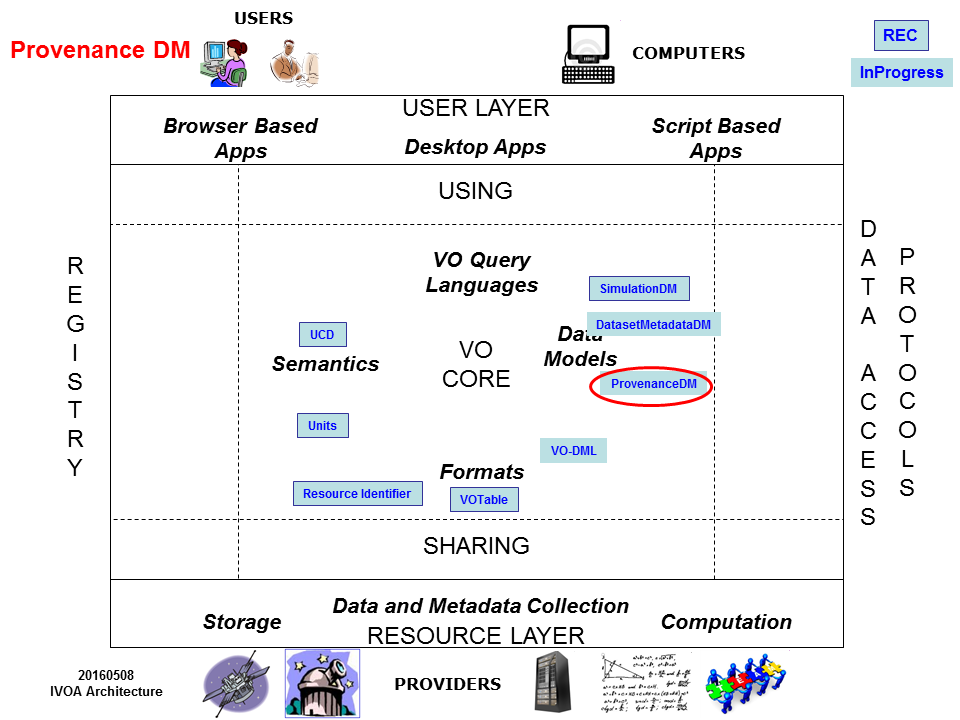
\includegraphics[width=\textwidth]{VOArchitecture-Prov2016.png}
\caption[Architecture diagram for the Provenance Data Model]{Architecture diagram for the Provenance Data Model. It is based on existing concepts defined in existing IVOA data models, and existing formats and semantics and fully integrated in the IVOA framework}
\label{fig:archdiag}
\end{figure}

Fig.~\ref{fig:archdiag} shows the dependencies of this document with respect to other existing standards.
%IVOA architecture \citep{note:VOARCH}.
